\documentclass[landscape]{article}
\usepackage[pdftex]{graphicx,color}
\pagestyle{empty}
\oddsidemargin  -0.5 in
\evensidemargin -0.5 in
\headheight     0 in
\topmargin      -1 in
\textheight     7.7 in
\textwidth      10 in
\begin{document}
\huge
\renewcommand{\labelitemi}{-}
\setlength{\parindent}{0 cm}

\mbox{ }

\vfill
\begin{center}\fbox{\begin{minipage}{0.95\linewidth}
    \vspace{0.5 cm}
    \begin{itemize}
      \item What is this talk about?
	\begin{itemize}

	  \item Efficiency of cuts for measuring $\displaystyle \int
	  \Upsilon \to$ hadrons

	  \item $\Upsilon \to \ell^+\ell^-$ are background, cascade
	  decays (even to $X \ell^+\ell^-$) are signal; \\ other
	  backgrounds are continuum processes, cosmic rays, beam-gas.

	\end{itemize}
      \end{itemize}
    \vspace{0.5 cm}
\end{minipage}}\end{center}

\vfill
\begin{center}\fbox{\begin{minipage}{0.95\linewidth}
    \vspace{0.5 cm}
    \begin{itemize}
      \item What's new since last time?
	\begin{itemize}
	  \item Several data/MC disagreement puzzles have been solved

	  \item A bug in EvtGen has been discovered (and fixed by Anders)

	  \item Most of the systematic error table has been filled in

	\end{itemize}
      \end{itemize}
    \vspace{0.5 cm}
\end{minipage}}\end{center}

\vfill
\begin{center} Jim Pivarski \end{center}

\vfill
\pagebreak

Hadronic efficiencies for each cut: $\Upsilon(1S)$
\vspace{1 cm}

\begin{tabular}{p{18 cm} p{6 cm}}
  $\left. \mbox{\begin{minipage}{\linewidth}\includegraphics[height=4 cm, width=\linewidth]{white.pdf}\end{minipage}} \right.$ & \begin{minipage}{\linewidth} \end{minipage} \\
  $\left. \mbox{\begin{minipage}{\linewidth}\includegraphics[height=0.7 cm, width=\linewidth]{white.pdf}\end{minipage}} \right.$ & \begin{minipage}{\linewidth} \end{minipage} \\
  $\left. \mbox{\begin{minipage}{\linewidth}\includegraphics[height=4.1 cm, width=\linewidth]{white.pdf}\end{minipage}} \right.$ & \begin{minipage}{\linewidth} \end{minipage}
\end{tabular}
\vspace{-9.7 cm}

\hspace{-0.75 cm}\includegraphics[width=0.5\linewidth, angle=-90]{all1_bblumi_normcc.pdf}

\begin{itemize}

\vfill
  \item \textcolor{blue}{Blue} diamonds are Monte Carlo, \textcolor{red}{red} boxes are data $\pm$ {\it stat} $\pm$ {\it syst}

\vfill
  \item Cuts are applied cumulatively

\vfill
  \item Data is $\Upsilon(1S)$ (from random on-resonance runs) \\

  \vspace{-0.7\baselineskip}
  \hspace{1 cm} \begin{minipage}{0.9\linewidth} $-$
  continuum (random off-res) $-$ beam-gas (single-beam runs) \\ $-$
  cosmic rays (no-beam runs) $-$ $\Upsilon(1S) \to \tau^+ \tau^-$ (from
  Monte Carlo) \end{minipage}

\end{itemize}

\vfill
\pagebreak

Hadronic efficiencies for each cut: $\Upsilon(2S)$
\vspace{1 cm}

\begin{tabular}{p{18 cm} p{6 cm}}
  $\left. \mbox{\begin{minipage}{\linewidth}\includegraphics[height=4 cm, width=\linewidth]{white.pdf}\end{minipage}} \right.$ & \begin{minipage}{\linewidth} \end{minipage} \\
  $\left. \mbox{\begin{minipage}{\linewidth}\includegraphics[height=0.7 cm, width=\linewidth]{white.pdf}\end{minipage}} \right.$ & \begin{minipage}{\linewidth} \end{minipage} \\
  $\left. \mbox{\begin{minipage}{\linewidth}\includegraphics[height=4.1 cm, width=\linewidth]{white.pdf}\end{minipage}} \right.$ & \begin{minipage}{\linewidth} \end{minipage}
\end{tabular}
\vspace{-9.7 cm}

\hspace{-0.75 cm}\includegraphics[width=0.5\linewidth, angle=-90]{all2_bblumi_normcc.pdf}

\begin{itemize}

\vfill
  \item \textcolor{blue}{Blue} diamonds are Monte Carlo, \textcolor{red}{red} boxes are data $\pm$ {\it stat} $\pm$ {\it syst}

\vfill
  \item Cuts are applied cumulatively

\vfill
  \item Data is $\Upsilon(2S)$ (from random on-resonance runs) \\

  \vspace{-0.7\baselineskip}
  \hspace{1 cm} \begin{minipage}{0.9\linewidth} $-$
  continuum (random off-res) $-$ beam-gas (single-beam runs) \\ $-$
  cosmic rays (no-beam runs) $-$ $\Upsilon(2S) \to \tau^+ \tau^-$ (from
  Monte Carlo) \end{minipage}

\end{itemize}

\vfill
\pagebreak

Hadronic efficiencies for each cut: $\Upsilon(3S)$
\vspace{1 cm}

\begin{tabular}{p{18 cm} p{6 cm}}
  $\left. \mbox{\begin{minipage}{\linewidth}\includegraphics[height=4 cm, width=\linewidth]{white.pdf}\end{minipage}} \right.$ & \begin{minipage}{\linewidth} \end{minipage} \\
  $\left. \mbox{\begin{minipage}{\linewidth}\includegraphics[height=0.7 cm, width=\linewidth]{white.pdf}\end{minipage}} \right.$ & \begin{minipage}{\linewidth} \end{minipage} \\
  $\left. \mbox{\begin{minipage}{\linewidth}\includegraphics[height=4.1 cm, width=\linewidth]{white.pdf}\end{minipage}} \right.$ & \begin{minipage}{\linewidth} \end{minipage}
\end{tabular}
\vspace{-9.7 cm}

\hspace{-0.75 cm}\includegraphics[width=0.5\linewidth, angle=-90]{all3_bblumi_normcc.pdf}

\begin{itemize}

\vfill
  \item \textcolor{blue}{Blue} diamonds are Monte Carlo, \textcolor{red}{red} boxes are data $\pm$ {\it stat} $\pm$ {\it syst}

\vfill
  \item Cuts are applied cumulatively

\vfill
  \item Data is $\Upsilon(3S)$ (from random on-resonance runs) \\

  \vspace{-0.7\baselineskip}
  \hspace{1 cm} \begin{minipage}{0.9\linewidth} $-$
  continuum (random off-res) $-$ beam-gas (single-beam runs) \\ $-$
  cosmic rays (no-beam runs) $-$ $\Upsilon(3S) \to \tau^+ \tau^-$ (from
  Monte Carlo) \end{minipage}

\end{itemize}

\vfill
\pagebreak

Here's how I will measure efficiency (you're looking at $\Upsilon(1S)$)
\vspace{1 cm}

\begin{tabular}{p{18 cm} p{6 cm}}
  $\left. \mbox{\begin{minipage}{\linewidth}\includegraphics[height=4 cm, width=\linewidth]{green.pdf}\end{minipage}} \right\}$ & \begin{minipage}{\linewidth} from Monte Carlo \end{minipage} \\
  $\left. \mbox{\begin{minipage}{\linewidth}\includegraphics[height=0.7 cm, width=\linewidth]{white.pdf}\end{minipage}} \right.$ & \begin{minipage}{\linewidth} from $\Upsilon(1S)$ data \end{minipage} \\
  $\left. \mbox{\begin{minipage}{\linewidth}\includegraphics[height=4.1 cm, width=\linewidth]{yellow.pdf}\end{minipage}} \right\}$ & \begin{minipage}{\linewidth} from data \end{minipage}
\end{tabular}
\vspace{-9.7 cm}

\hspace{-0.75 cm}\includegraphics[width=0.5\linewidth, angle=-90]{all1_bblumi_normcc.pdf}

\begin{itemize}

\vfill
  \item Fraction that passes first four cuts ($\epsilon_{MC}$) is
  calculated from Monte Carlo; \\ data is used to bound systematic
  errors

\vfill
  \item Fraction that passes Z cut ($\epsilon_Z$) is calculated from
  $\Upsilon(1S)$ data and applied to all three

\vfill
  \item Fraction that passes last four cuts ($\epsilon_{data}$) is
  calculated from data for each resonance

\end{itemize}

\begin{center} $\epsilon_{total} = \epsilon_{MC} \mbox{ }\cdot\mbox{ } \epsilon_Z \mbox{ }\cdot\mbox{ } \epsilon_{data}$ \end{center}

\pagebreak

\begin{tabular}{p{0.6\linewidth} p{0.4\linewidth}}
  \begin{minipage}{\linewidth}
    \begin{tabular}{p{0.47\linewidth} p{0.43\linewidth}}
      \begin{minipage}{\linewidth}\begin{center} $\Upsilon(1S)$ \end{center}\end{minipage} &
      \begin{minipage}{\linewidth}\includegraphics[height=0.2\textheight]{cheat_sheet.pdf}\end{minipage}
    \end{tabular}
    \hspace{0.25 cm} \includegraphics[height=0.75\textheight]{all1_bblumi_normcc_trigger.pdf}
  \end{minipage} &
  \hspace{-1.5 cm}
  \begin{minipage}{1.1\linewidth}

    \begin{itemize}

      \item Trigger requirement is
	\begin{center} Hadron OR RadTau OR ElTrack \end{center}
	{\Large
	Hadron = $\ge$3 AXIAL tracks AND $\ge$1 CBLO \\
	RadTau = $\ge$2 STEREO tracks AND \\
        \mbox{\hspace{4 cm}} ($\ge$2 CBLO OR $\ge$1 CBMD) \\
	ElTrack = $\ge$1 AXIAL track AND $\ge$1 CBMD} \\

      \item MC efficiency of trigger is 99.5\%

\vspace{0.75 cm}
      \color{black} \item Shifting CBMD=0 bin to match data changes efficiency by 0.01\%

\vspace{0.75 cm}
      \item Shifting CBLO=7 bin to match data changes efficiency by 0.02\%

\vspace{0.75 cm}
      \color{black} \item Work in progress: testing for lost events by looking at
      correlations between triggers and with TwoTrack

    \end{itemize}

  \end{minipage}
\end{tabular}

\begin{tabular}{p{0.6\linewidth} p{0.4\linewidth}}
  \begin{minipage}{\linewidth}
    \begin{tabular}{p{0.47\linewidth} p{0.43\linewidth}}
      \begin{minipage}{\linewidth}\begin{center} $\Upsilon(2S)$ \end{center}\end{minipage} &
      \begin{minipage}{\linewidth}\includegraphics[height=0.2\textheight]{cheat_sheet.pdf}\end{minipage}
    \end{tabular}
    \hspace{0.25 cm} \includegraphics[height=0.75\textheight]{all2_bblumi_normcc_trigger.pdf}
  \end{minipage} &
  \hspace{-1.5 cm}
  \begin{minipage}{1.1\linewidth}

    \begin{itemize}

      \item Trigger requirement is
	\begin{center} Hadron OR RadTau OR ElTrack \end{center}
	{\Large
	Hadron = $\ge$3 AXIAL tracks AND $\ge$1 CBLO \\
	RadTau = $\ge$2 STEREO tracks AND \\
        \mbox{\hspace{4 cm}} ($\ge$2 CBLO OR $\ge$1 CBMD) \\
	ElTrack = $\ge$1 AXIAL track AND $\ge$1 CBMD} \\

      \item MC efficiency of trigger is 99.5\%

\vspace{0.75 cm}
      \color{white} \item Shifting CBMD=0 bin to match data changes efficiency by 0.01\%

\vspace{0.75 cm}
      \item Shifting CBLO=7 bin to match data changes efficiency by 0.02\%

\vspace{0.75 cm}
      \color{black} \item Work in progress: testing for lost events by
      looking at correlations between triggers and with TwoTrack

    \end{itemize}

  \end{minipage} \\
\end{tabular}

\begin{tabular}{p{0.6\linewidth} p{0.4\linewidth}}
  \begin{minipage}{\linewidth}
    \begin{tabular}{p{0.47\linewidth} p{0.43\linewidth}}
      \begin{minipage}{\linewidth}\begin{center} $\Upsilon(3S)$ \end{center}\end{minipage} &
      \begin{minipage}{\linewidth}\includegraphics[height=0.2\textheight]{cheat_sheet.pdf}\end{minipage}
    \end{tabular}
    \hspace{0.25 cm} \includegraphics[height=0.75\textheight]{all3_bblumi_normcc_trigger.pdf}
  \end{minipage} &
  \hspace{-1.5 cm}
  \begin{minipage}{1.1\linewidth}

    \begin{itemize}

      \item Trigger requirement is
	\begin{center} Hadron OR RadTau OR ElTrack \end{center}
	{\Large
	Hadron = $\ge$3 AXIAL tracks AND $\ge$1 CBLO \\
	RadTau = $\ge$2 STEREO tracks AND \\
        \mbox{\hspace{4 cm}} ($\ge$2 CBLO OR $\ge$1 CBMD) \\
	ElTrack = $\ge$1 AXIAL track AND $\ge$1 CBMD} \\

      \item MC efficiency of trigger is 99.5\%

\vspace{0.75 cm}
      \color{white} \item Shifting CBMD=0 bin to match data changes efficiency by 0.01\%

\vspace{0.75 cm}
      \item Shifting CBLO=7 bin to match data changes efficiency by 0.02\%

\vspace{0.75 cm}
      \color{black} \item Work in progress: testing for lost events by looking at
      correlations between triggers and with TwoTrack

    \end{itemize}

  \end{minipage}
\end{tabular}

\begin{tabular}{p{0.6\linewidth} p{0.4\linewidth}}
  \begin{minipage}{\linewidth}
    \begin{tabular}{p{0.9\linewidth} p{0.1 cm}}
      \begin{minipage}{\linewidth}\begin{center} $\Upsilon(2S) \to \pi^+\pi^- \Upsilon(1S)$ \mbox{\hspace{6 cm}} \\
\vspace{0.25\baselineskip} \mbox{\hspace{4.9 cm}} $\Upsilon(1S) \to$ 0, 1, 2 extra tracks\end{center}\end{minipage} &
      \begin{minipage}{\linewidth}\includegraphics[height=0.2\textheight, width=0.1 cm]{white.pdf}\end{minipage}
    \end{tabular}
    \hspace{0.25 cm} \includegraphics[height=0.75\textheight, clip=false]{final_cascades.pdf}
  \end{minipage} &
  \hspace{-1.5 cm}
  \begin{minipage}{1.1\linewidth}

    \begin{itemize}

      \item $\Upsilon(2S) \to \pi^+\pi^-\Upsilon(1S)$ can be used to
      check for missing physics in the Monte Carlo

\vspace{1 cm}
      \item Here, $\pi^+$ and $\pi^-$ satisfy
	\begin{center} 2 STEREO tracks and 2 CBLO \\
	  2 reconstructed tracks \end{center}

\vspace{1 cm}
      \item The rest of the $\Upsilon(1S)$ must satisfy \\
	{\Large
	  Visible energy $>$ 20\% center-of-mass \\
	  Total CC energy $<$ 85\% center-of-mass \\
	  Biggest shower energy $<$ 85\% beam \\
	  2nd-biggest track momentum $<$ 85\% beam}

\vspace{1 cm}
      \item Data and MC are normalized at 2-track bin to $\Upsilon(1S)
      \to$ 2 tracks (3.05\%, mostly $\tau^+\tau^-$ and hadrons)

\vspace{1 cm}
      \item Uncertainty in agreement introduces $\pm$0.07\% trigger
      systematic


    \end{itemize}

  \end{minipage}
\end{tabular}

\begin{tabular}{p{0.6\linewidth} p{0.4\linewidth}}
  \begin{minipage}{\linewidth}
    \begin{tabular}{p{0.47\linewidth} p{0.43\linewidth}}
      \begin{minipage}{\linewidth}\begin{center} $\Upsilon(1S)$ \end{center}\end{minipage} &
      \begin{minipage}{\linewidth}\includegraphics[height=0.2\textheight]{cheat_sheet.pdf}\end{minipage}
    \end{tabular}
    \hspace{0.25 cm} \includegraphics[height=0.75\textheight]{all1_bblumi_normcc_d0close.pdf}
  \end{minipage} &
  \hspace{-1.5 cm}
  \begin{minipage}{1.1\linewidth}

    \begin{itemize}

      \item Trigger has already required one track, use its distance
      {\it from the beamspot} to cut out cosmic rays

      \vspace{1 cm}

      \item MC efficiency is 99.90\%

      \vspace{1 cm}

      \item If this cut is moved out to infinity or in to 2 mm,
      efficiency changes by $\pm$0.25\%

    \end{itemize}

  \end{minipage}
\end{tabular}

\begin{tabular}{p{0.6\linewidth} p{0.4\linewidth}}
  \begin{minipage}{\linewidth}
    \begin{tabular}{p{0.47\linewidth} p{0.43\linewidth}}
      \begin{minipage}{\linewidth}\begin{center} $\Upsilon(2S)$ \end{center}\end{minipage} &
      \begin{minipage}{\linewidth}\includegraphics[height=0.2\textheight]{cheat_sheet.pdf}\end{minipage}
    \end{tabular}
    \hspace{0.25 cm} \includegraphics[height=0.75\textheight]{all2_bblumi_normcc_d0close.pdf}
  \end{minipage} &
  \hspace{-1.5 cm}
  \begin{minipage}{1.1\linewidth}

    \begin{itemize}

      \item Trigger has already required one track, use its distance
      {\it from the beamspot} to cut out cosmic rays

      \vspace{1 cm}

      \item MC efficiency is 99.90\%

      \vspace{1 cm}

      \item If this cut is moved out to infinity or in to 2 mm,
      efficiency changes by $\pm$0.25\%

    \end{itemize}

  \end{minipage}
\end{tabular}

\begin{tabular}{p{0.6\linewidth} p{0.4\linewidth}}
  \begin{minipage}{\linewidth}
    \begin{tabular}{p{0.47\linewidth} p{0.43\linewidth}}
      \begin{minipage}{\linewidth}\begin{center} $\Upsilon(3S)$ \end{center}\end{minipage} &
      \begin{minipage}{\linewidth}\includegraphics[height=0.2\textheight]{cheat_sheet.pdf}\end{minipage}
    \end{tabular}
    \hspace{0.25 cm} \includegraphics[height=0.75\textheight]{all3_bblumi_normcc_d0close.pdf}
  \end{minipage} &
  \hspace{-1.5 cm}
  \begin{minipage}{1.1\linewidth}

    \begin{itemize}

      \item Trigger has already required one track, use its distance
      {\it from the beamspot} to cut out cosmic rays

      \vspace{1 cm}

      \item MC efficiency is 99.90\%

      \vspace{1 cm}

      \item If this cut is moved out to infinity or in to 2 mm,
      efficiency changes by $\pm$0.25\%

    \end{itemize}

  \end{minipage} \\
\end{tabular}

\begin{tabular}{p{0.6\linewidth} p{0.4\linewidth}}
  \begin{minipage}{\linewidth}
    \begin{tabular}{p{0.47\linewidth} p{0.43\linewidth}}
      \begin{minipage}{\linewidth}\begin{center} $\Upsilon(1S)$ \end{center}\end{minipage} &
      \begin{minipage}{\linewidth}\includegraphics[height=0.2\textheight]{cheat_sheet.pdf}\end{minipage}
    \end{tabular}
    \hspace{0.25 cm} 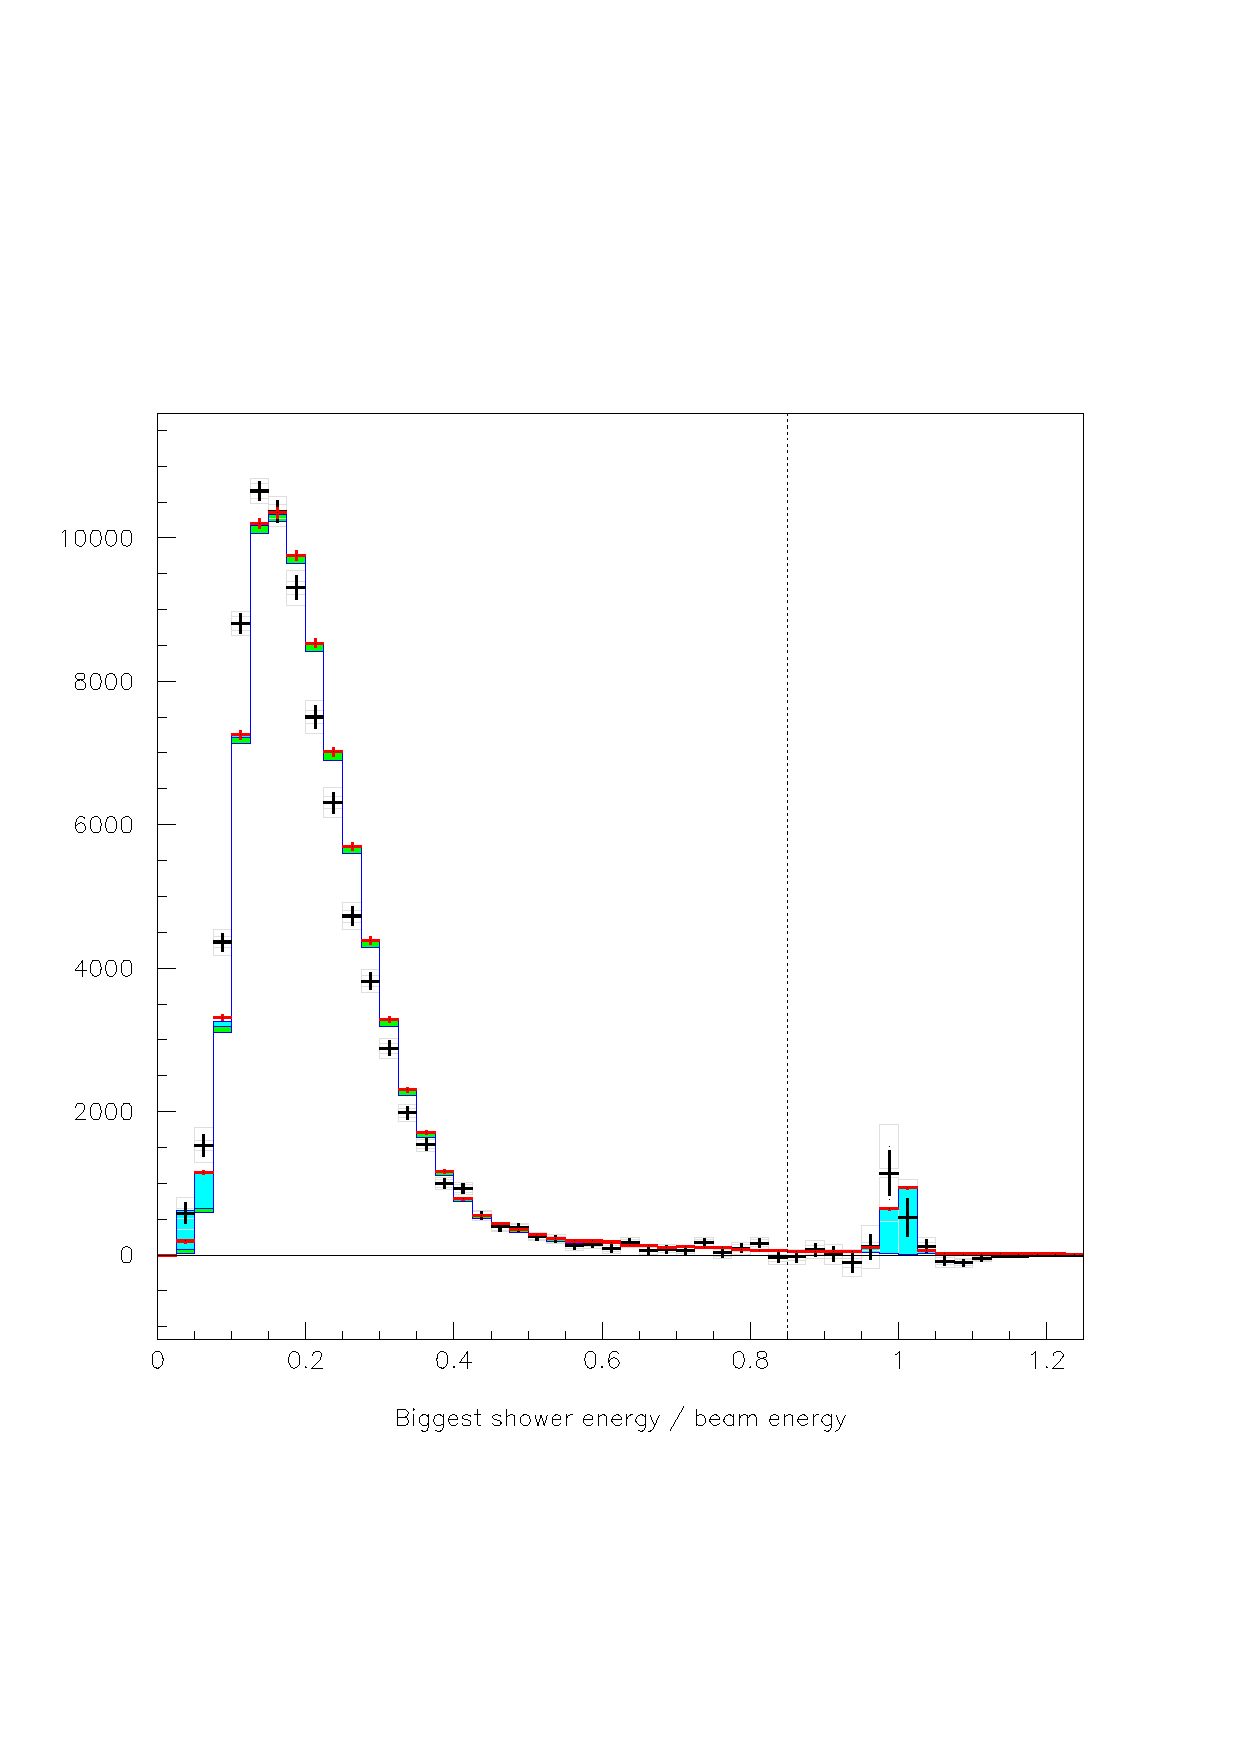
\includegraphics[height=0.75\textheight]{superplots_all1_e1.pdf}
  \end{minipage} &
  \hspace{-1.5 cm}
  \begin{minipage}{1.1\linewidth}

    \begin{itemize}

      \item Little $\Upsilon(1S) \to e^+e^-$ peak is a background

\vspace{1 cm}
      \item $gg\gamma$ span the cut boundary, all other hadrons are well to the left

\vspace{1 cm}
      \item $\Gamma_{gg\gamma}/\Gamma_{ggg}$ is precise? \\
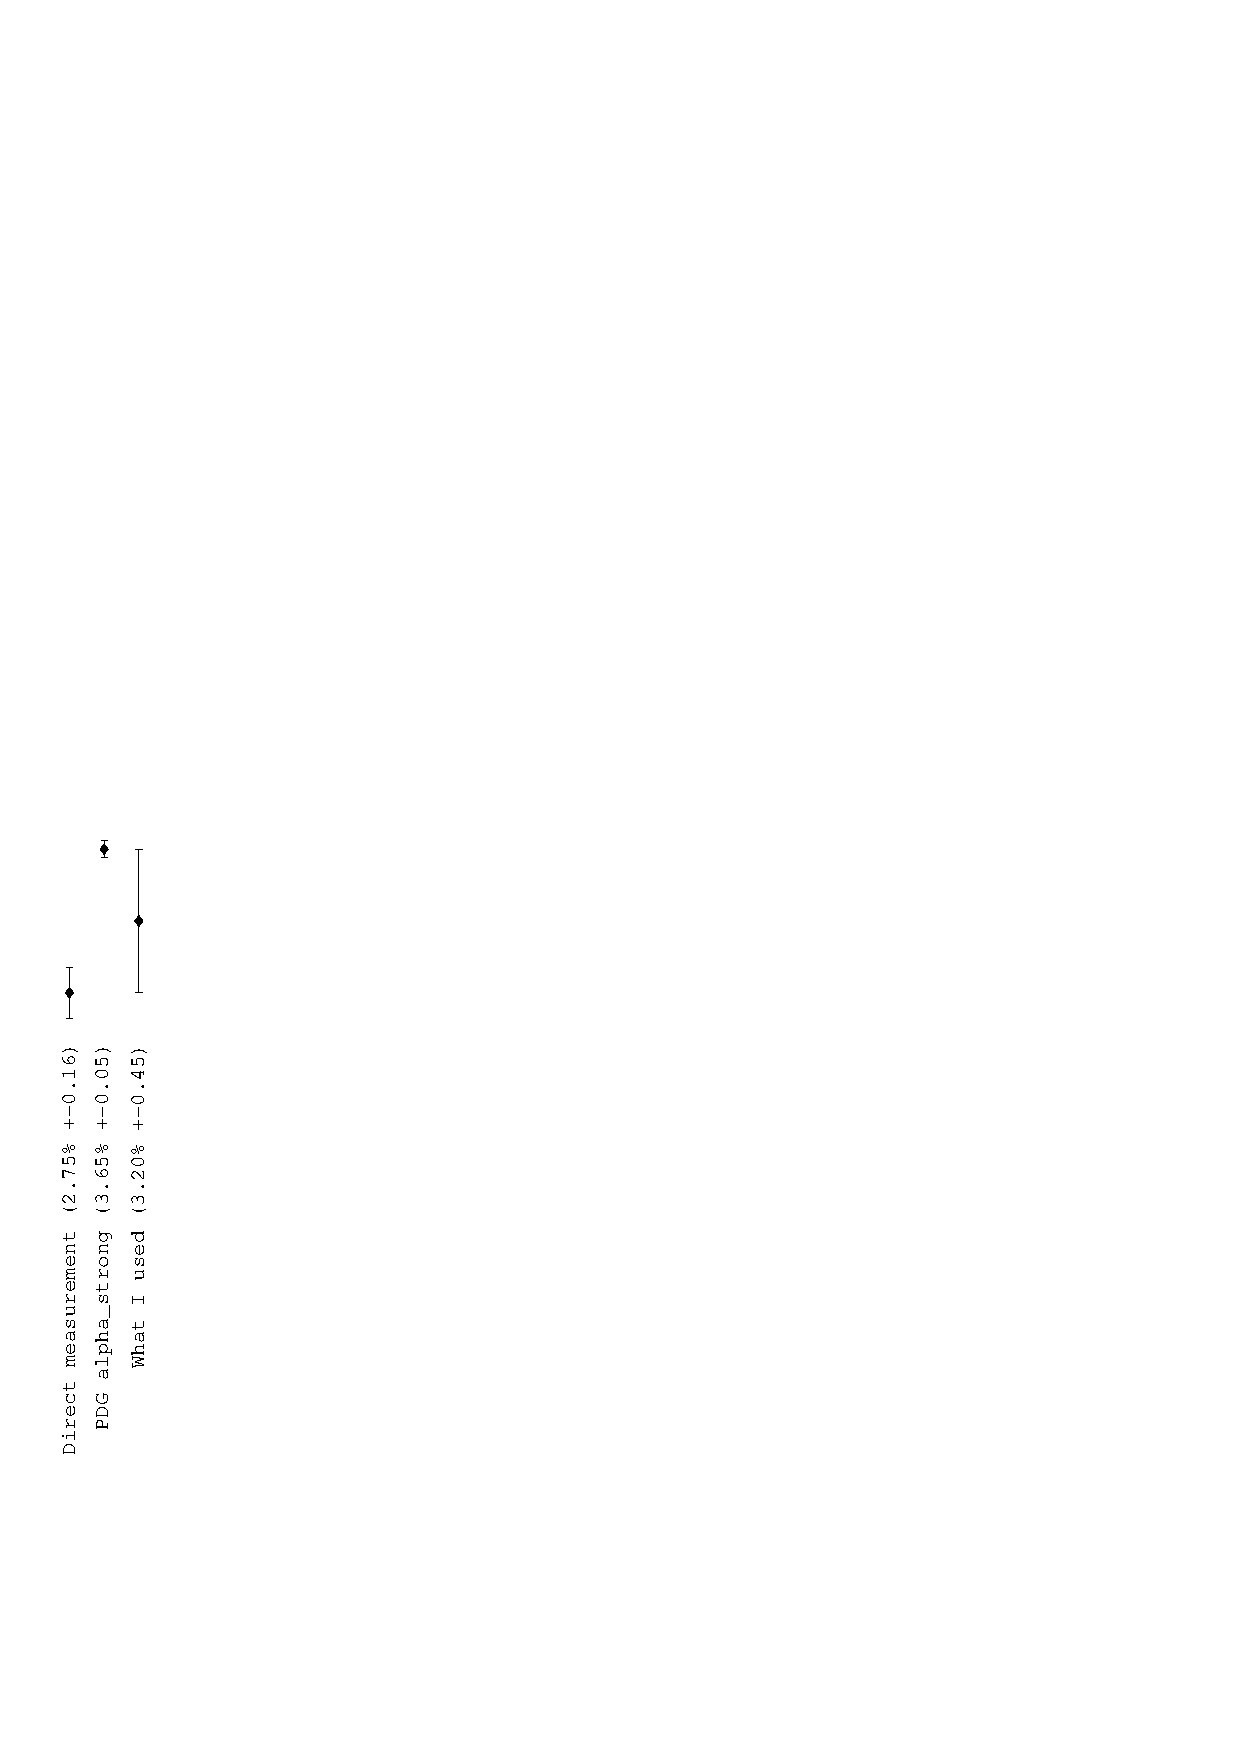
\includegraphics[height=\linewidth, angle=-90, bb=30 160 100 440]{alphas_used.pdf}

\vspace{0.5 cm}
      \item Introduces $\pm$0.08\% systematic

    \end{itemize}

  \end{minipage} \\
\end{tabular}

\begin{tabular}{p{0.6\linewidth} p{0.4\linewidth}}
  \begin{minipage}{\linewidth}
    \begin{tabular}{p{0.47\linewidth} p{0.43\linewidth}}
      \begin{minipage}{\linewidth}\begin{center} Aside: EvtGen Bug \end{center}\end{minipage} &
      \begin{minipage}{\linewidth}\includegraphics[height=0.2\textheight, width=0.1 cm]{white.pdf}\end{minipage}
    \end{tabular}
    \hspace{0.25 cm} \includegraphics[height=0.75\textheight]{example_big_gggamma.pdf}
  \end{minipage} &
  \hspace{-1.5 cm}
  \begin{minipage}{1.1\linewidth}

    \begin{itemize}

      \item $gg\gamma$ events were not modelled correctly in EvtGen:
      boost of $gg$ was done in the wrong direction

\vspace{1 cm}
      \item This event had a 4 GeV photon on one side and 28 GeV of
      pileup on the other.  (Biggest shower distribution was distorted.)

\vspace{1 cm}
      \item For the purposes of this talk, $gg\gamma$ efficiency is
      measured from {\tt QQ}.

\vspace{1 cm}
      \item Bug is corrected in
	\begin{center} EvtGenModels {\tt v01\_02\_01} \end{center}

    \end{itemize}

  \end{minipage} \\
\end{tabular}

\begin{tabular}{p{0.6\linewidth} p{0.4\linewidth}}
  \begin{minipage}{\linewidth}
    \begin{tabular}{p{0.47\linewidth} p{0.43\linewidth}}
      \begin{minipage}{\linewidth}\begin{center} $\Upsilon(2S)$ \end{center}\end{minipage} &
      \begin{minipage}{\linewidth}\includegraphics[height=0.2\textheight]{cheat_sheet.pdf}\end{minipage}
    \end{tabular}
    \hspace{0.25 cm} 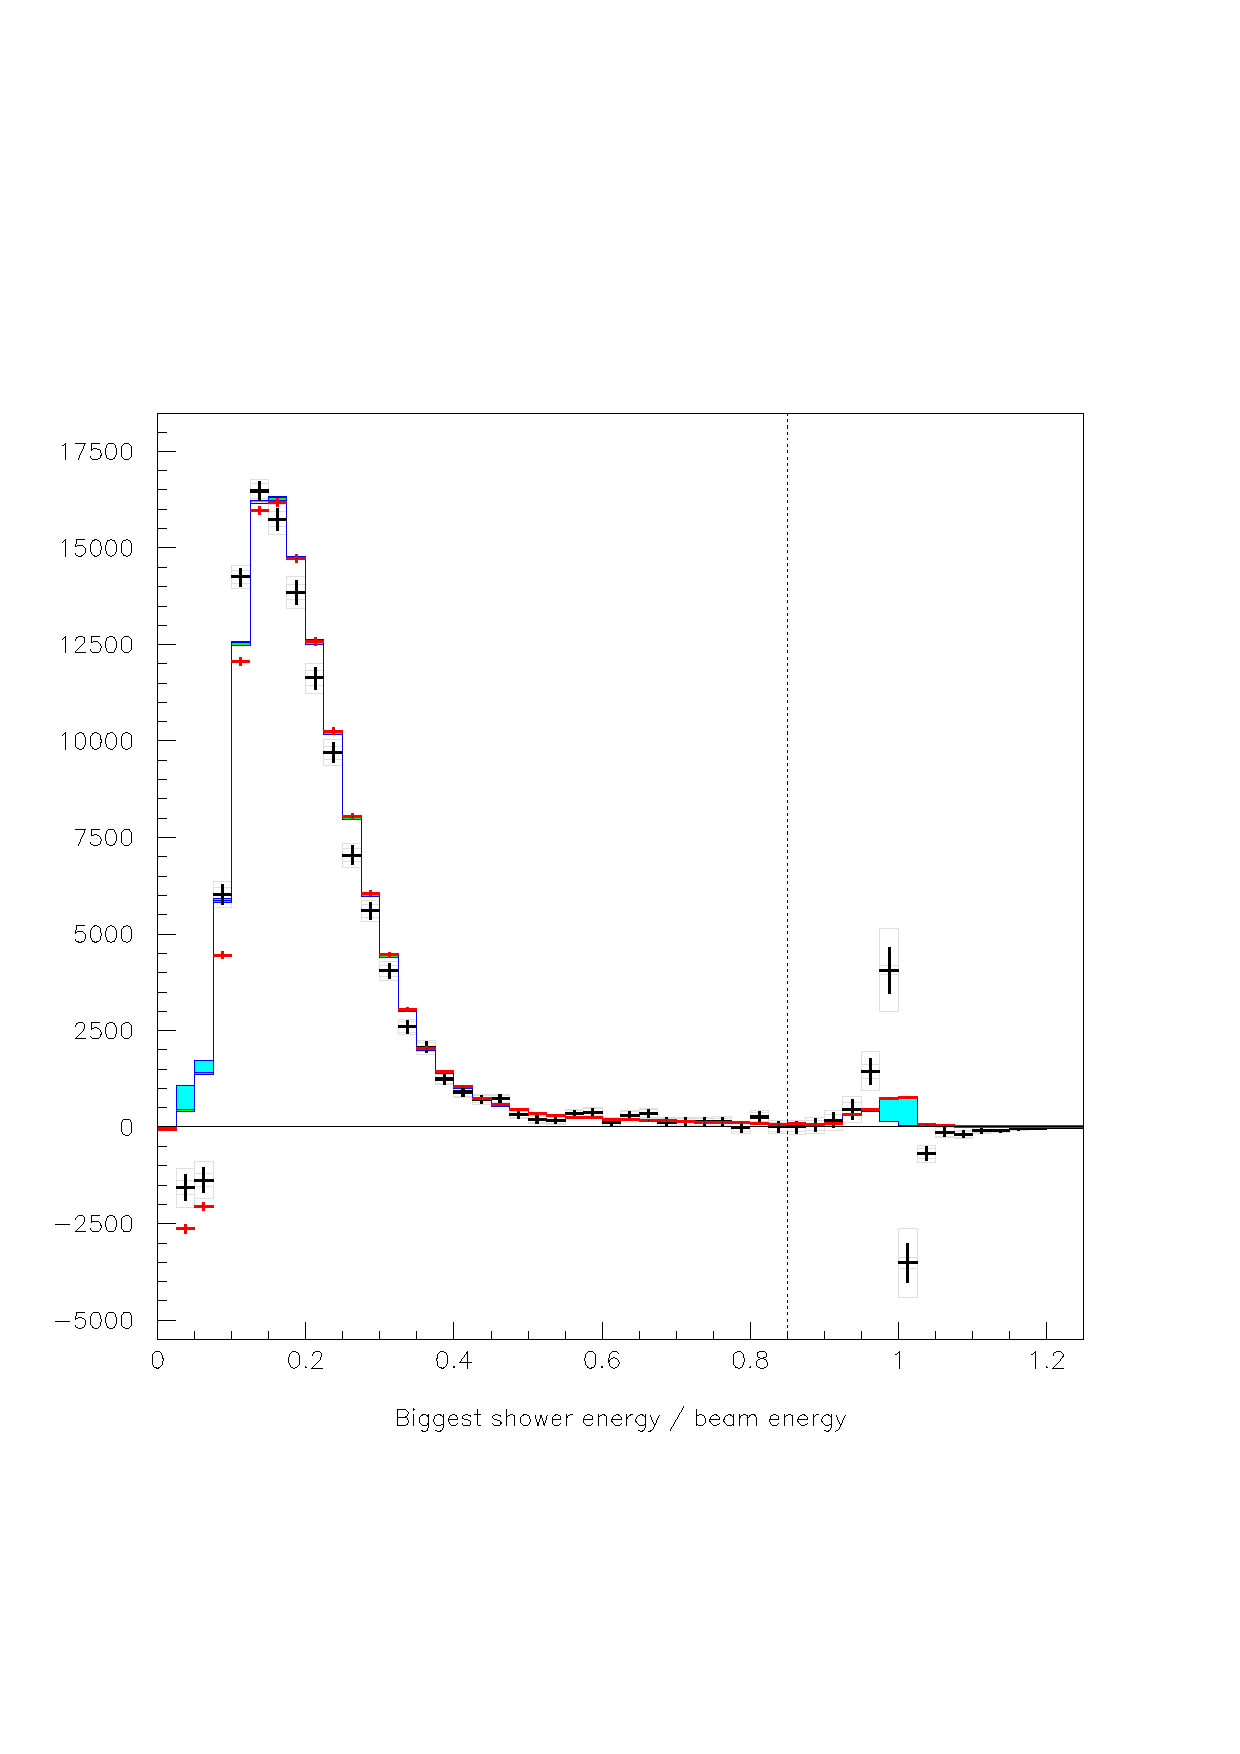
\includegraphics[height=0.75\textheight]{superplots_all2_e1.pdf}
  \end{minipage} &
  \hspace{-1.5 cm}
  \begin{minipage}{1.1\linewidth}

    \begin{itemize}

      \item Residuals add to zero on both sides of the cut threshold

\vspace{1 cm}
      \item Bhabha peak energy differs by 3 MeV between on- and off-resonance

\vspace{1 cm}
      \item Cascades to electrons (signal) are all to the right of the threshold

\vspace{1 cm}
      \item Vary $\mathcal{B}_{\mu\mu}$ and cascade $\mathcal{B}$'s by
      their uncertainties: $\pm$0.06\% in $\epsilon_{MC}$

\vspace{1 cm}
      \item Suppose {\tt PHOTOS} is 50\% wrong: $\pm$0.03\% in $\epsilon_{MC}$

    \end{itemize}

  \end{minipage} \\
\end{tabular}

\begin{tabular}{p{0.6\linewidth} p{0.4\linewidth}}
  \begin{minipage}{\linewidth}
    \begin{tabular}{p{0.47\linewidth} p{0.43\linewidth}}
      \begin{minipage}{\linewidth}\begin{center} $\Upsilon(3S)$ \end{center}\end{minipage} &
      \begin{minipage}{\linewidth}\includegraphics[height=0.2\textheight]{cheat_sheet.pdf}\end{minipage}
    \end{tabular}
    \hspace{0.25 cm} 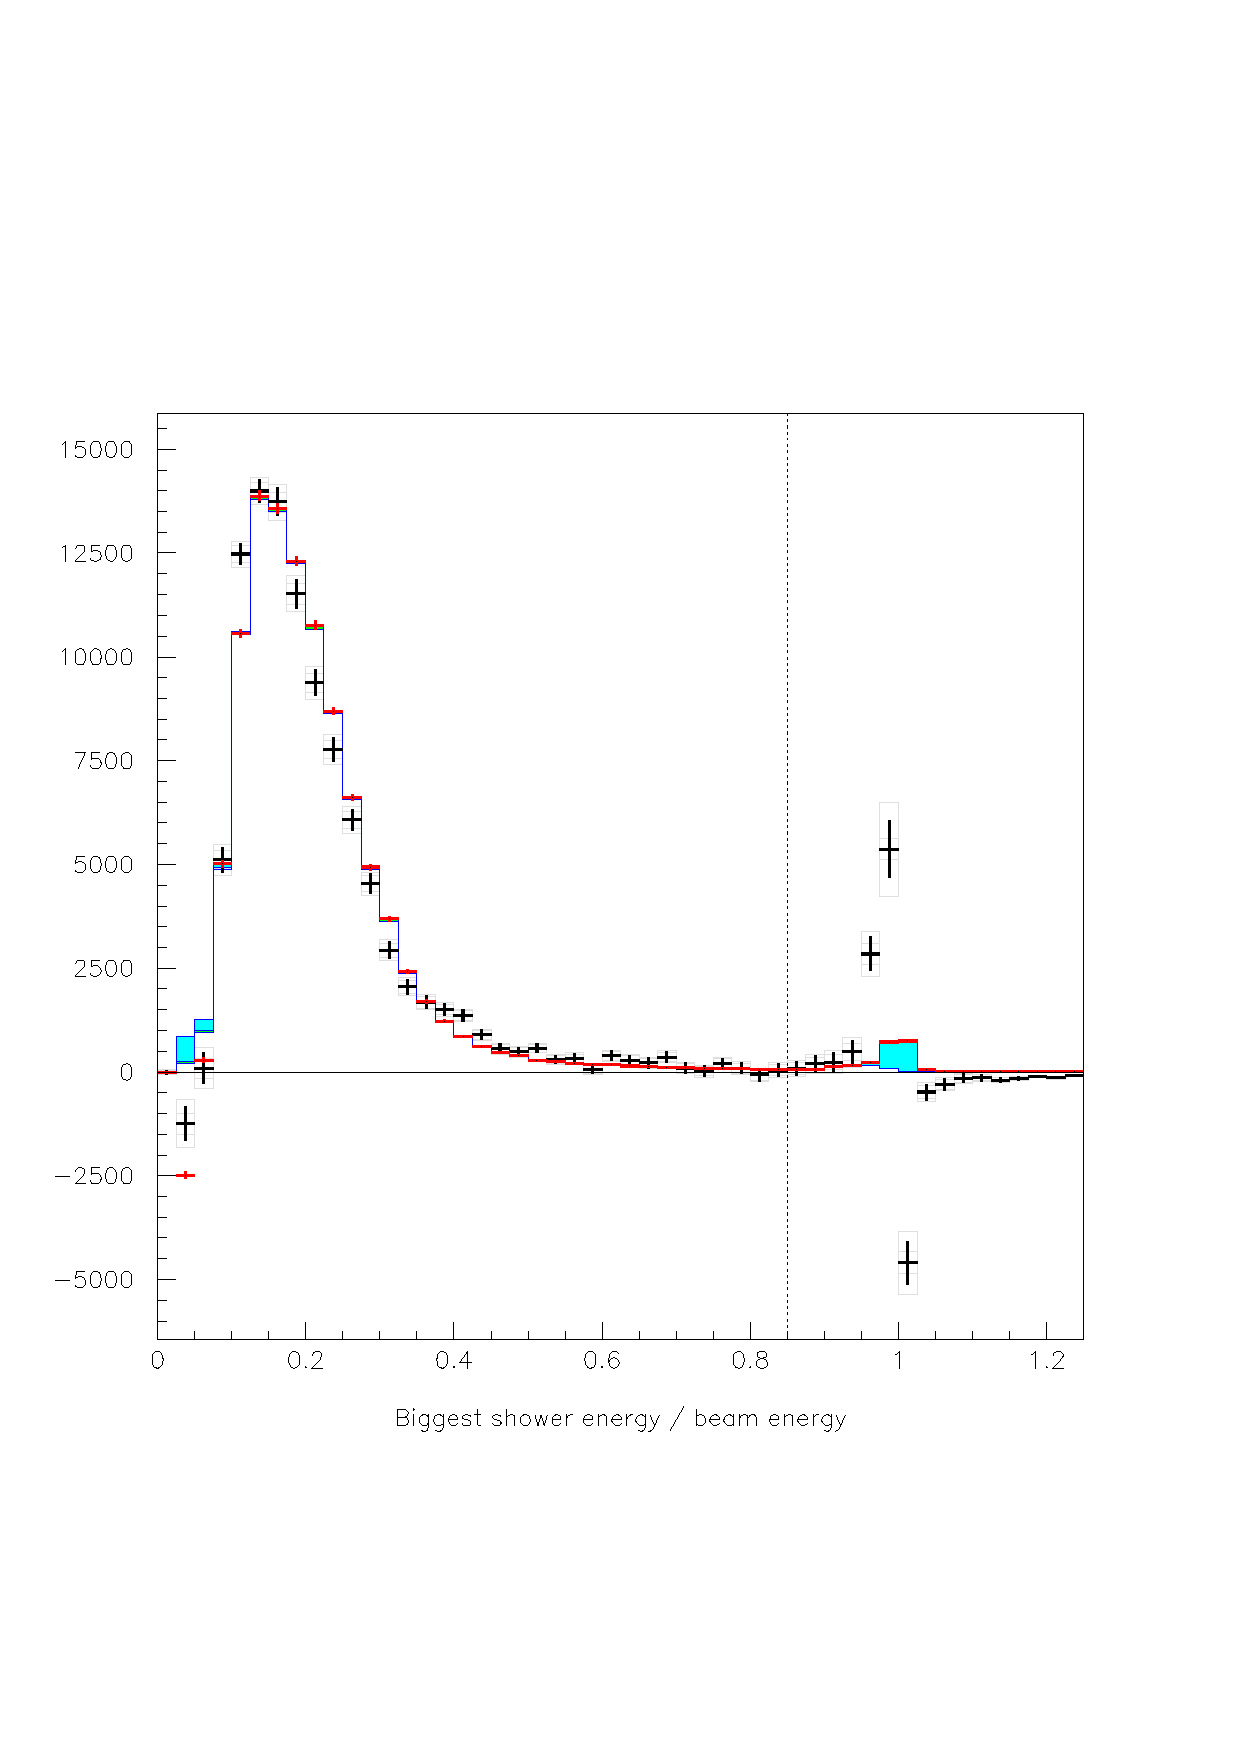
\includegraphics[height=0.75\textheight]{superplots_all3_e1.pdf}
  \end{minipage} &
  \hspace{-1.5 cm}
  \begin{minipage}{1.1\linewidth}

    \begin{itemize}

      \item Residuals add to zero on both sides of the cut threshold

\vspace{1 cm}
      \item Bhabha peak energy differs by 3 MeV between on- and off-resonance

\vspace{1 cm}
      \item Cascades to electrons (signal) are all to the right of the threshold

\vspace{1 cm}
      \item Vary $\mathcal{B}_{\mu\mu}$ and cascade $\mathcal{B}$'s by
      their uncertainties: $\pm$0.05\% in $\epsilon_{MC}$

\vspace{1 cm}
      \item Suppose {\tt PHOTOS} is 50\% wrong: $\pm$0.01\% in $\epsilon_{MC}$

    \end{itemize}

  \end{minipage} \\
\end{tabular}

\begin{tabular}{p{0.6\linewidth} p{0.4\linewidth}}
  \begin{minipage}{\linewidth}
    \begin{tabular}{p{0.47\linewidth} p{0.43\linewidth}}
      \begin{minipage}{\linewidth}\begin{center} $\Upsilon(1S)$ \end{center}\end{minipage} &
      \begin{minipage}{\linewidth}\includegraphics[height=0.2\textheight]{cheat_sheet.pdf}\end{minipage}
    \end{tabular}
    \hspace{0.25 cm} 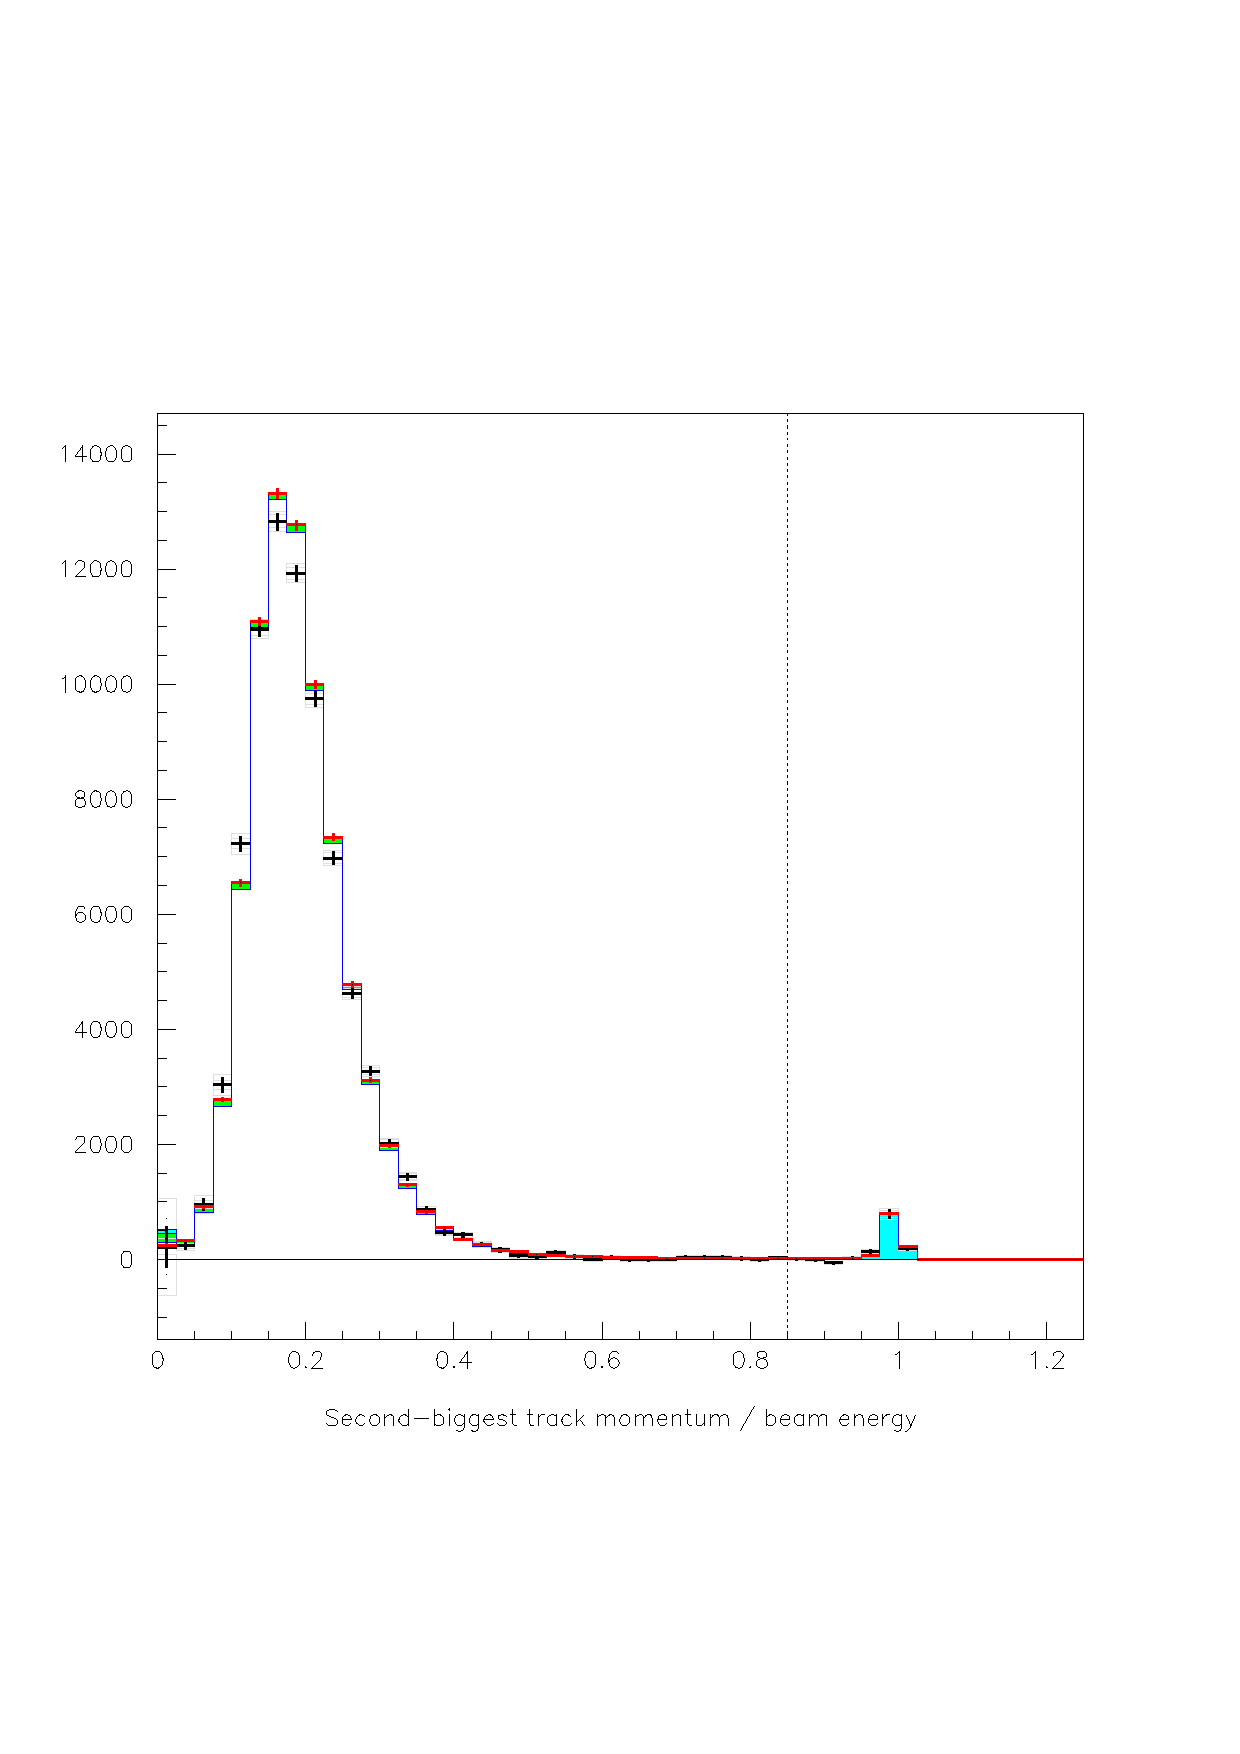
\includegraphics[height=0.75\textheight]{superplots_all1_p2.pdf}
  \end{minipage} &
  \hspace{-1.5 cm}
  \begin{minipage}{1.1\linewidth}

    \begin{itemize}

      \item If there is no second track, this is automatically satisfied

\vspace{1 cm}
      \color{white} \item $\mathcal{B}_{\mu\mu}$ in MC is 1.5\%, \\ Istvan found 2.03\% \color{black}

    \end{itemize}

  \end{minipage} \\
\end{tabular}

\begin{tabular}{p{0.6\linewidth} p{0.4\linewidth}}
  \begin{minipage}{\linewidth}
    \begin{tabular}{p{0.47\linewidth} p{0.43\linewidth}}
      \begin{minipage}{\linewidth}\begin{center} $\Upsilon(2S)$ \end{center}\end{minipage} &
      \begin{minipage}{\linewidth}\includegraphics[height=0.2\textheight]{cheat_sheet.pdf}\end{minipage}
    \end{tabular}
    \hspace{0.25 cm} 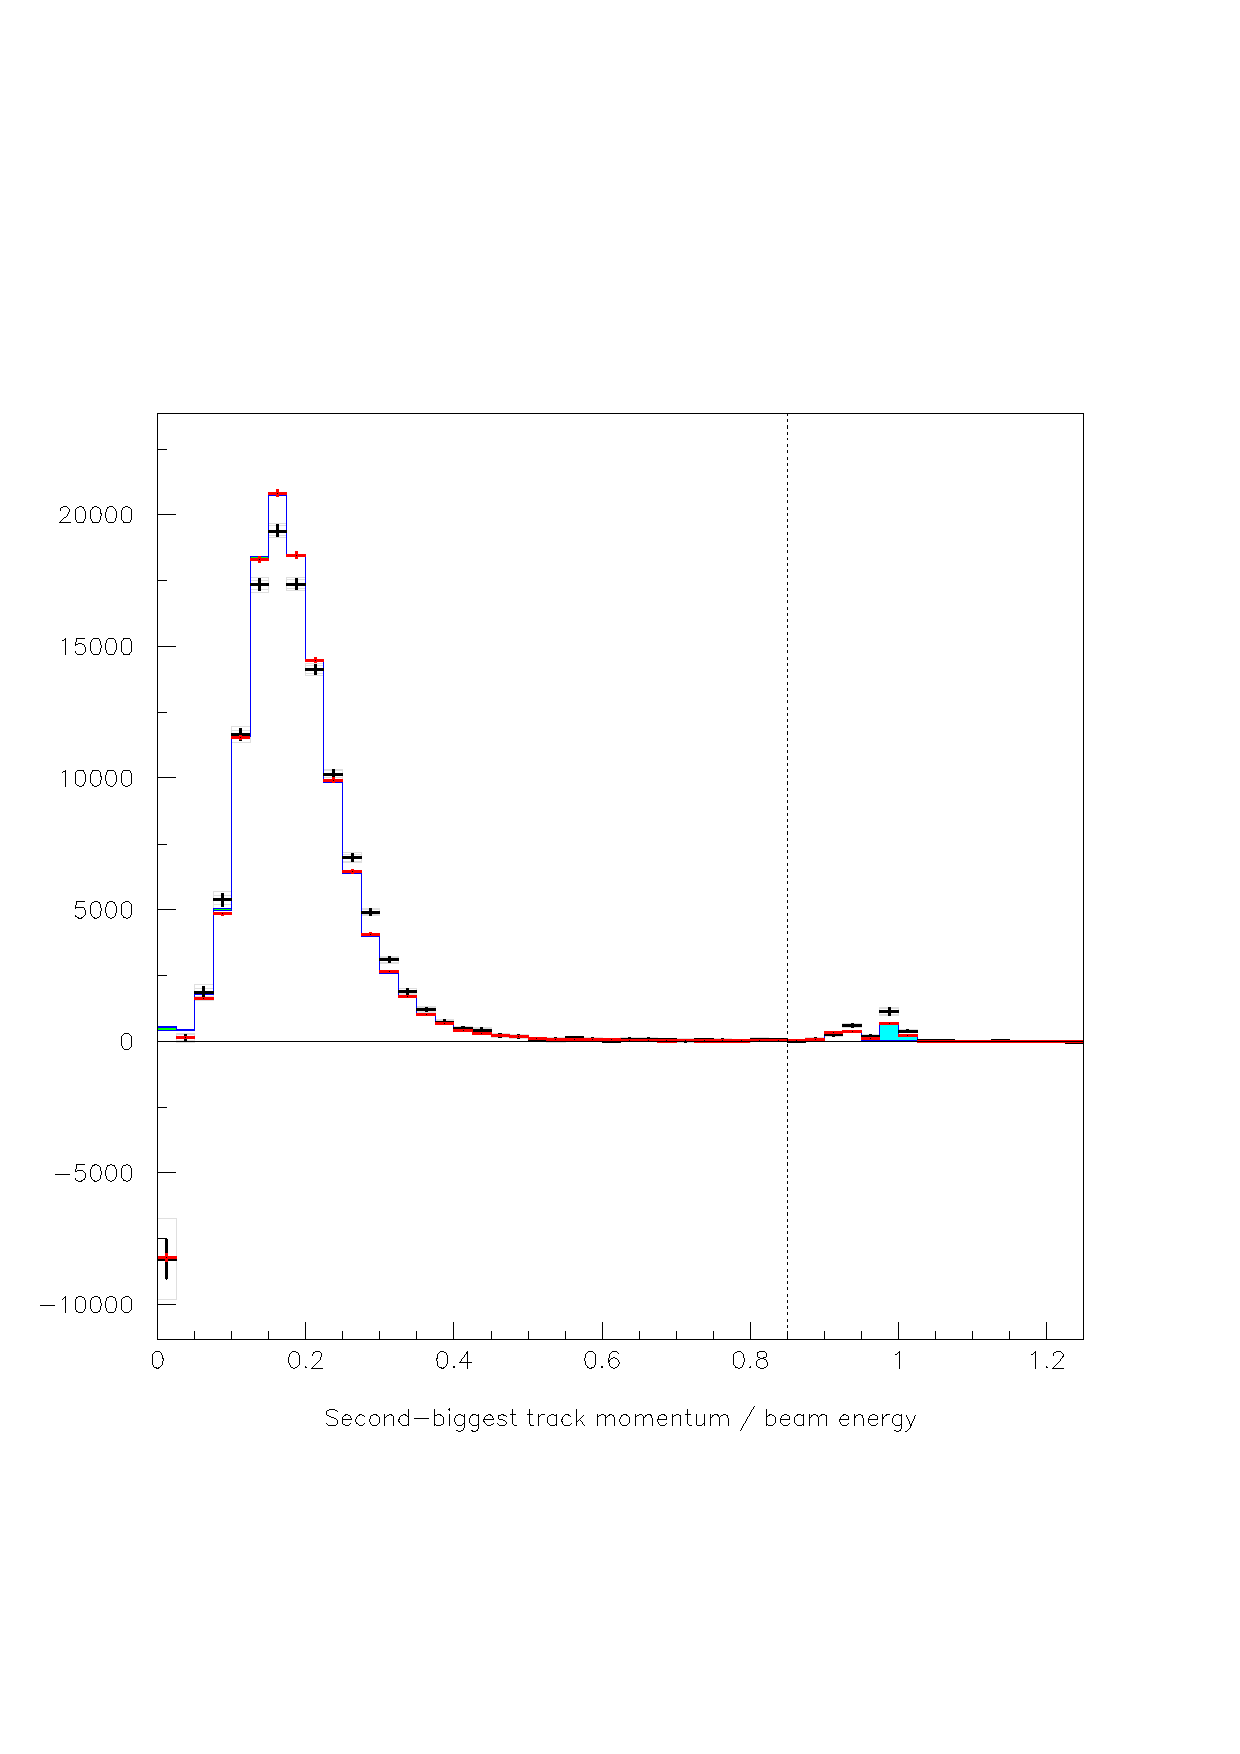
\includegraphics[height=0.75\textheight]{superplots_all2_p2.pdf}
  \end{minipage} &
  \hspace{-1.5 cm}
  \begin{minipage}{1.1\linewidth}

    \begin{itemize}

      \item If there is no second track, this is automatically satisfied

\vspace{1 cm}
      \color{black} \item $\mathcal{B}_{\mu\mu}$ in MC is 1.5\%, \\ Istvan found 2.03\%

    \end{itemize}

  \end{minipage} \\
\end{tabular}

\begin{tabular}{p{0.6\linewidth} p{0.4\linewidth}}
  \begin{minipage}{\linewidth}
    \begin{tabular}{p{0.47\linewidth} p{0.43\linewidth}}
      \begin{minipage}{\linewidth}\begin{center} $\Upsilon(3S)$ \end{center}\end{minipage} &
      \begin{minipage}{\linewidth}\includegraphics[height=0.2\textheight]{cheat_sheet.pdf}\end{minipage}
    \end{tabular}
    \hspace{0.25 cm} 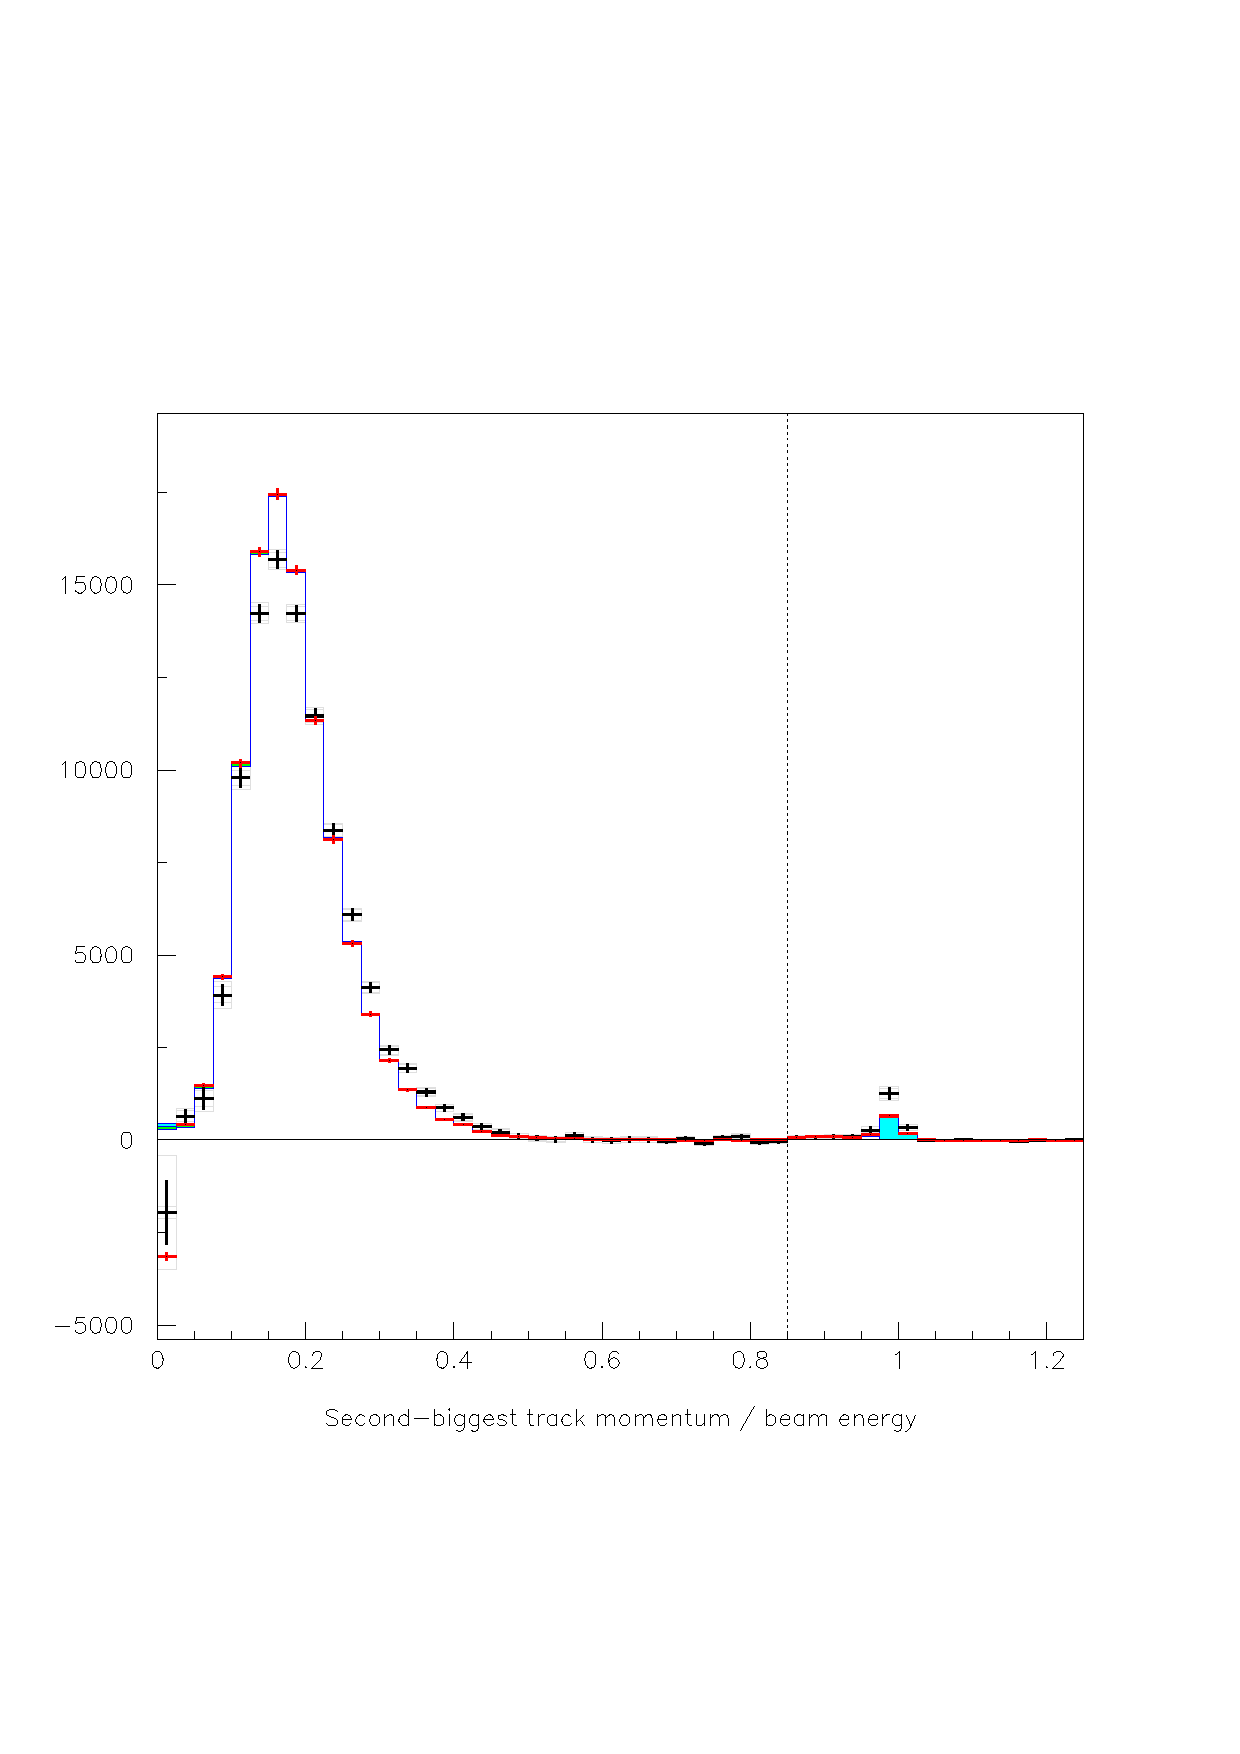
\includegraphics[height=0.75\textheight]{superplots_all3_p2.pdf}
  \end{minipage} &
  \hspace{-1.5 cm}
  \begin{minipage}{1.1\linewidth}

    \begin{itemize}

      \item If there is no second track, this is automatically satisfied

\vspace{1 cm}
      \color{black} \item $\mathcal{B}_{\mu\mu}$ in MC is 1.81\%, \\ Istvan found 2.39\%

    \end{itemize}

  \end{minipage} \\
\end{tabular}

\begin{tabular}{p{0.6\linewidth} p{0.4\linewidth}}
  \begin{minipage}{\linewidth}
    \begin{tabular}{p{0.47\linewidth} p{0.43\linewidth}}
      \begin{minipage}{\linewidth}\begin{center} $\Upsilon(1S)$ \end{center}\end{minipage} &
      \begin{minipage}{\linewidth}\includegraphics[height=0.2\textheight]{cheat_sheet.pdf}\end{minipage}
    \end{tabular}
    \hspace{0.25 cm} \includegraphics[height=0.75\textheight]{all1_bblumi_normcc_wz.pdf}
  \end{minipage} &
  \hspace{-1.5 cm}
  \begin{minipage}{1.1\linewidth}

    \begin{itemize}

      \item Suppress beamgas by cutting {\it around beamspot} in Z

\vspace{1 cm}
      \item Fallback on closest track z0 is included to keep from
      implicitly requiring two tracks (I forgot to move z0 to the
      beamspot)

\vspace{1 cm}
      \item Efficiency of this cut is measured from $\Upsilon(1S)$ data:
\begin{center} 99.35\% $\pm$ 0.20\% $\pm$ 0.56\% \end{center}

\begin{tabular}{p{3 cm} p{2.5 cm} p{2.5 cm}}
&
\begin{minipage}{\linewidth} \begin{center}
    $\uparrow$ \\
    \it sample stat
\end{center} \end{minipage} &
\begin{minipage}{\linewidth} \begin{center}
    $\uparrow$ \\
    \it scaling error
\end{center} \end{minipage}
\end{tabular}
\vspace{-2 cm}

    \end{itemize}

  \end{minipage} \\
\end{tabular}

\begin{tabular}{p{0.6\linewidth} p{0.4\linewidth}}
  \begin{minipage}{\linewidth}
    \begin{tabular}{p{0.47\linewidth} p{0.43\linewidth}}
      \begin{minipage}{\linewidth}\begin{center} $\Upsilon(2S)$ \end{center}\end{minipage} &
      \begin{minipage}{\linewidth}\includegraphics[height=0.2\textheight]{cheat_sheet.pdf}\end{minipage}
    \end{tabular}
    \hspace{0.25 cm} \includegraphics[height=0.75\textheight]{all2_bblumi_normcc_wz.pdf}
  \end{minipage} &
  \hspace{-1.5 cm}
  \begin{minipage}{1.1\linewidth}

    \begin{itemize}

      \item Suppress beamgas by cutting {\it around beamspot} in Z

\vspace{1 cm}
      \item Fallback on closest track z0 is included to keep from
      implicitly requiring two tracks (I forgot to move z0 to the
      beamspot)

\vspace{1 cm}
      \item Efficiency of this cut is measured from $\Upsilon(1S)$ data:
\begin{center} 99.35\% $\pm$ 0.20\% $\pm$ 0.56\% \end{center}

\begin{tabular}{p{3 cm} p{2.5 cm} p{2.5 cm}}
&
\begin{minipage}{\linewidth} \begin{center}
    $\uparrow$ \\
    \it sample stat
\end{center} \end{minipage} &
\begin{minipage}{\linewidth} \begin{center}
    $\uparrow$ \\
    \it scaling error
\end{center} \end{minipage}
\end{tabular}
\vspace{-2 cm}

    \end{itemize}

  \end{minipage} \\
\end{tabular}

\begin{tabular}{p{0.6\linewidth} p{0.4\linewidth}}
  \begin{minipage}{\linewidth}
    \begin{tabular}{p{0.47\linewidth} p{0.43\linewidth}}
      \begin{minipage}{\linewidth}\begin{center} $\Upsilon(3S)$ \end{center}\end{minipage} &
      \begin{minipage}{\linewidth}\includegraphics[height=0.2\textheight]{cheat_sheet.pdf}\end{minipage}
    \end{tabular}
    \hspace{0.25 cm} \includegraphics[height=0.75\textheight]{all3_bblumi_normcc_wz.pdf}
  \end{minipage} &
  \hspace{-1.5 cm}
  \begin{minipage}{1.1\linewidth}

    \begin{itemize}

      \item Suppress beamgas by cutting {\it around beamspot} in Z

\vspace{1 cm}
      \item Fallback on closest track z0 is included to keep from
      implicitly requiring two tracks (I forgot to move z0 to the
      beamspot)

\vspace{1 cm}
      \item Efficiency of this cut is measured from $\Upsilon(1S)$ data:
\begin{center} 99.35\% $\pm$ 0.20\% $\pm$ 0.56\% \end{center}

\begin{tabular}{p{3 cm} p{2.5 cm} p{2.5 cm}}
&
\begin{minipage}{\linewidth} \begin{center}
    $\uparrow$ \\
    \it sample stat
\end{center} \end{minipage} &
\begin{minipage}{\linewidth} \begin{center}
    $\uparrow$ \\
    \it scaling error
\end{center} \end{minipage}
\end{tabular}
\vspace{-2 cm}

    \end{itemize}

  \end{minipage} \\
\end{tabular}

\begin{tabular}{p{0.6\linewidth} p{0.4\linewidth}}
  \begin{minipage}{\linewidth}
    \begin{tabular}{p{0.47\linewidth} p{0.43\linewidth}}
      \begin{minipage}{\linewidth}\begin{center} $\Upsilon(1S)$ \end{center}\end{minipage} &
      \begin{minipage}{\linewidth}\includegraphics[height=0.2\textheight]{cheat_sheet.pdf}\end{minipage}
    \end{tabular}
    \hspace{0.25 cm} \includegraphics[height=0.75\textheight]{superplots_all1_visen.pdf}
  \end{minipage} &
  \hspace{-1.5 cm}
  \begin{minipage}{1.1\linewidth}

    \begin{itemize}

      \item Efficiency is measured from data:
\begin{center} 99.29\% $\pm$ 0.33\% $\pm$ 0.75\% \end{center}

\vspace{1 cm}
      \item Residual below threshold sums to zero, within errors (280
      $\pm$ 350)

\vspace{1 cm}
      \item Bin on top of cosmic ray peak is 2.6$\sigma$ high

    \end{itemize}

  \end{minipage} \\
\end{tabular}

\begin{tabular}{p{0.6\linewidth} p{0.4\linewidth}}
  \begin{minipage}{\linewidth}
    \begin{tabular}{p{0.47\linewidth} p{0.43\linewidth}}
      \begin{minipage}{\linewidth}\begin{center} $\Upsilon(2S)$ \end{center}\end{minipage} &
      \begin{minipage}{\linewidth}\includegraphics[height=0.2\textheight]{cheat_sheet.pdf}\end{minipage}
    \end{tabular}
    \hspace{0.25 cm} \includegraphics[height=0.75\textheight]{superplots_all2_visen.pdf}
  \end{minipage} &
  \hspace{-1.5 cm}
  \begin{minipage}{1.1\linewidth}

    \begin{itemize}

      \item Efficiency is measured from data:
\begin{center} 98.05\% $\pm$ 0.41\% $\pm$ 0.83\% \end{center}

\vspace{1 cm}
      \item Residual below threshold sums to 1840 $\pm$ 720

\vspace{1 cm}
      \item Bin at top of cosmic ray peak is 3.3$\sigma$ high: scaling
      cosmics incorrectly?

    \end{itemize}

  \end{minipage} \\
\end{tabular}

\begin{tabular}{p{0.6\linewidth} p{0.4\linewidth}}
  \begin{minipage}{\linewidth}
    \begin{tabular}{p{0.47\linewidth} p{0.43\linewidth}}
      \begin{minipage}{\linewidth}\begin{center} $\Upsilon(3S)$ \end{center}\end{minipage} &
      \begin{minipage}{\linewidth}\includegraphics[height=0.2\textheight]{cheat_sheet.pdf}\end{minipage}
    \end{tabular}
    \hspace{0.25 cm} \includegraphics[height=0.75\textheight]{superplots_all3_visen.pdf}
  \end{minipage} &
  \hspace{-1.5 cm}
  \begin{minipage}{1.1\linewidth}

    \begin{itemize}

      \item Efficiency is measured from data:
\begin{center} 99.99\% $\pm$ 0.54\% $\pm$ 1.07\% \end{center}

\vspace{1 cm}
      \item Residual below threshold sums to zero (-380 $\pm$ 850)

\vspace{1 cm}
      \item But that wiggle is getting out of hand!

    \end{itemize}

  \end{minipage} \\
\end{tabular}

\pagebreak

No wiggle without hot showers

\vfill

\begin{center}
  \begin{tabular}{p{0.45\linewidth} p{0.45\linewidth}}
    \includegraphics[width=0.9\linewidth]{normcc_visen.pdf} &
    \includegraphics[width=0.9\linewidth]{coolcc_visen.pdf}
  \end{tabular}

  \begin{tabular}{p{0.45\linewidth} p{0.45\linewidth}}
    \begin{minipage}{\linewidth} \begin{center} Normal visible energy \end{center} \end{minipage} &
    \begin{minipage}{\linewidth} \begin{center} No hot showers \end{center} \end{minipage}
  \end{tabular}
\end{center}

\vfill

\begin{itemize}

  \item Bottom plots are before continuum subtraction: there's a large
  peak of continuum processes (look like two-photon events) below the
  35\% of center-of-mass energy cut.

\vfill
  \item Difference in hot showers between on- and off-resonance shifts
  one peak 23 MeV relative to the other

\vfill
  \item This answers $\Upsilon(1S)$ and $\Upsilon(3S)$ discrepancies,
  but not $\Upsilon(2S)$.

\end{itemize}

\vfill

\pagebreak

\begin{tabular}{p{0.6\linewidth} p{0.4\linewidth}}
  \begin{minipage}{\linewidth}
    \begin{tabular}{p{0.47\linewidth} p{0.43\linewidth}}
      \begin{minipage}{\linewidth}\begin{center} $\Upsilon(1S)$ \end{center}\end{minipage} &
      \begin{minipage}{\linewidth}\includegraphics[height=0.2\textheight]{cheat_sheet.pdf}\end{minipage}
    \end{tabular}
    \hspace{0.25 cm} \includegraphics[height=0.75\textheight]{all1_bblumi_normcc_tracks.pdf}
  \end{minipage} &
  \hspace{-1.5 cm}
  \begin{minipage}{1.1\linewidth}

    \begin{itemize}

      \item Efficiency is measured from data:
\begin{center} 100.35\% $\pm$ 0.17\% $\pm$ 0.30\% \end{center}

\vspace{1 cm}
      \item Data/MC disagreement no longer matters because I'm
      not using MC

    \end{itemize}

  \end{minipage} \\
\end{tabular}

\begin{tabular}{p{0.6\linewidth} p{0.4\linewidth}}
  \begin{minipage}{\linewidth}
    \begin{tabular}{p{0.47\linewidth} p{0.43\linewidth}}
      \begin{minipage}{\linewidth}\begin{center} $\Upsilon(2S)$ \end{center}\end{minipage} &
      \begin{minipage}{\linewidth}\includegraphics[height=0.2\textheight]{cheat_sheet.pdf}\end{minipage}
    \end{tabular}
    \hspace{0.25 cm} \includegraphics[height=0.75\textheight]{all2_bblumi_normcc_tracks.pdf}
  \end{minipage} &
  \hspace{-1.5 cm}
  \begin{minipage}{1.1\linewidth}

    \begin{itemize}

      \item Efficiency is measured from data:
\begin{center} 100.22\% $\pm$ 0.22\% $\pm$ 0.39\% \end{center}

\vspace{1 cm}
      \item Data/MC disagreement no longer matters because I'm
      not using MC

    \end{itemize}

  \end{minipage} \\
\end{tabular}

\begin{tabular}{p{0.6\linewidth} p{0.4\linewidth}}
  \begin{minipage}{\linewidth}
    \begin{tabular}{p{0.47\linewidth} p{0.43\linewidth}}
      \begin{minipage}{\linewidth}\begin{center} $\Upsilon(3S)$ \end{center}\end{minipage} &
      \begin{minipage}{\linewidth}\includegraphics[height=0.2\textheight]{cheat_sheet.pdf}\end{minipage}
    \end{tabular}
    \hspace{0.25 cm} \includegraphics[height=0.75\textheight]{all3_bblumi_normcc_tracks.pdf}
  \end{minipage} &
  \hspace{-1.5 cm}
  \begin{minipage}{1.1\linewidth}

    \begin{itemize}

      \item Efficiency is measured from data:
\begin{center} 99.31\% $\pm$ 0.29\% $\pm$ 0.51\% \end{center}

\vspace{1 cm}
      \item Data/MC disagreement no longer matters because I'm
      not using MC

    \end{itemize}

  \end{minipage} \\
\end{tabular}

\begin{tabular}{p{0.6\linewidth} p{0.4\linewidth}}
  \begin{minipage}{\linewidth}
    \begin{tabular}{p{0.47\linewidth} p{0.43\linewidth}}
      \begin{minipage}{\linewidth}\begin{center} $\Upsilon(1S)$ \end{center}\end{minipage} &
      \begin{minipage}{\linewidth}\includegraphics[height=0.2\textheight]{cheat_sheet.pdf}\end{minipage}
    \end{tabular}
    \hspace{0.25 cm} \includegraphics[height=0.75\textheight]{superplots_all1_ccen.pdf}
  \end{minipage} &
  \hspace{-1.5 cm}
  \begin{minipage}{1.1\linewidth}

    \begin{itemize}

      \item Efficiency is measured from data:
\begin{center} 99.85\% $\pm$ 0.09\% $\pm$ 0.26\% \end{center}

\vspace{1 cm}
      \item Data/MC disagreement no longer matters because I'm
      not using MC

    \end{itemize}

  \end{minipage} \\
\end{tabular}

\begin{tabular}{p{0.6\linewidth} p{0.4\linewidth}}
  \begin{minipage}{\linewidth}
    \begin{tabular}{p{0.47\linewidth} p{0.43\linewidth}}
      \begin{minipage}{\linewidth}\begin{center} $\Upsilon(2S)$ \end{center}\end{minipage} &
      \begin{minipage}{\linewidth}\includegraphics[height=0.2\textheight]{cheat_sheet.pdf}\end{minipage}
    \end{tabular}
    \hspace{0.25 cm} \includegraphics[height=0.75\textheight]{superplots_all2_ccen.pdf}
  \end{minipage} &
  \hspace{-1.5 cm}
  \begin{minipage}{1.1\linewidth}

    \begin{itemize}

      \item Efficiency is measured from data:
\begin{center} 99.63\% $\pm$ 0.11\% $\pm$ 0.32\% \end{center}

\vspace{1 cm}
      \item Data/MC disagreement no longer matters because I'm
      not using MC

    \end{itemize}

  \end{minipage} \\
\end{tabular}

\begin{tabular}{p{0.6\linewidth} p{0.4\linewidth}}
  \begin{minipage}{\linewidth}
    \begin{tabular}{p{0.47\linewidth} p{0.43\linewidth}}
      \begin{minipage}{\linewidth}\begin{center} $\Upsilon(3S)$ \end{center}\end{minipage} &
      \begin{minipage}{\linewidth}\includegraphics[height=0.2\textheight]{cheat_sheet.pdf}\end{minipage}
    \end{tabular}
    \hspace{0.25 cm} \includegraphics[height=0.75\textheight]{superplots_all3_ccen.pdf}
  \end{minipage} &
  \hspace{-1.5 cm}
  \begin{minipage}{1.1\linewidth}

    \begin{itemize}

      \item Efficiency is measured from data:
\begin{center} 99.45\% $\pm$ 0.15\% $\pm$ 0.42\% \end{center}

\vspace{1 cm}
      \item Data/MC disagreement no longer matters because I'm
      not using MC

    \end{itemize}

  \end{minipage} \\
\end{tabular}

\pagebreak

\begin{center}
  \begin{tabular}{p{0.6\linewidth} r r r r}
    & \mbox{\hspace{0.3 cm}} & $\Upsilon(1S)$ & $\Upsilon(2S)$ & $\Upsilon(3S)$ \\\hline\hline
    \begin{minipage}{\linewidth} \begin{center} $\epsilon_{MC}$ \end{center} \end{minipage} & & 99.03\% & 97.62\% & 98.24\% \\
    what's the trigger uncertainty?  all of itself? & & $\sim$ 0.50\% & $\sim$ 0.50\% & $\sim$ 0.50\% \\
    limit on untriggerable zero-track events & & $\pm$ 0.07\% & $\pm$ 0.07\% & $\pm$ 0.07\% \\
    closest track to beamspot & & $\pm$ 0.25\% & $\pm$ 0.25\% & $\pm$ 0.25\% \\
    $gg\gamma$ events straddle biggest-shower energy threshold & & $\pm$ 0.09\% & $\pm$ 0.08\% & $\pm$ 0.08\% \\
    \begin{minipage}{\linewidth} cascade decays to $e^+e^-$ fail biggest shower cut, \\ cascade decays to $\mu^+\mu^-$ fail second-biggest track cut \end{minipage} & & & $\pm$ 0.06\% & $\pm$ 0.05\% \\
    assume {\tt PHOTOS} to be 50\% wrong & & & $\pm$ 0.03\% & $\pm$ 0.01\% \\
    Peter Onyisi's EvtGen-bunchfinder bug & & $\pm$ 0.17\% & $\pm$ 0.30\% & $\pm$ 0.13\% \\
    \begin{minipage}{\linewidth} I need to generate separate $\Upsilon \to q\bar{q}$ samples with the right branching fractions, but here are some bounds I placed on how much difference that will make \end{minipage} \vspace{0.05 cm} & & $<$ 0.19\% & $<$ 0.44\% & $<$ 0.44\% \\\hline
    \begin{minipage}{\linewidth} \begin{center} $\epsilon_{Z}$ \end{center} \end{minipage} & & 99.35\% & 99.35\% & 99.35\% \\
    sample statistics & & $\pm$ 0.20\% & $\pm$ 0.20\% & $\pm$ 0.20\% \\
    scaling systematics & & $\pm$ 0.56\% & $\pm$ 0.56\% & $\pm$ 0.56\% \\\hline
    \begin{minipage}{\linewidth} \begin{center} $\epsilon_{data}$ \end{center} \end{minipage} & & 99.49\% & 97.92\% & 98.74\% \\
    sample statistics (combined) & & $\pm$ 0.34\% & $\pm$ 0.39\% & $\pm$ 0.55\% \\
    scaling systematics (combined) & & $\pm$ 0.81\% & $\pm$ 0.88\% & $\pm$ 1.10\% \\\hline\hline
    & & 97.88\% & 94.97\% & 96.37\% \\
    \begin{minipage}{\linewidth} \begin{center} Totals \end{center} \end{minipage} & & $\pm$ 0.39\% & $\pm$ 0.44\% & $\pm$ 0.59\% \\
    & & $\pm$ 1.15\% & $\pm$ 1.30\% & $\pm$ 1.44\% \\
  \end{tabular}
\end{center}






\end{document}

%% \vfill
%% \begin{center}\fbox{\begin{minipage}{0.95\linewidth}
%%     \vspace{0.5 cm}
%%     \begin{itemize}
%%       \item What more will be needed before I can report a final
%%       result for the number of $\Upsilon$'s in CLEO-III?
%% 	\begin{itemize}
%% 	  \item I need to understand the trigger efficiency better

%% 	  \item I need to generate Monte Carlo to handle mode
%% 	  uncertainties correctly
%% 	\end{itemize}
%%       \end{itemize}
%%     \vspace{0.5 cm}
%% \end{minipage}}\end{center}

%% \vfill
%% \begin{center}\fbox{\begin{minipage}{0.95\linewidth}
%%     \vspace{0.5 cm}
%%     \begin{itemize}
%%       \item What more will be needed before I can report $\Gamma_{ee}$?
%% 	\begin{itemize}
%% 	  \item I need to (personally) understand the luminosity measurement

%% 	  \item Fitting, lineshape studies, and upper bounds on energy
%% 	  fluctuations
%% 	\end{itemize}
%%       \end{itemize}
%%     \vspace{0.5 cm}
%% \end{minipage}}\end{center}
